\section{Introduction}

With the rapid emergence of large language models (LLMs), evaluation benchmarks have become increasingly critical, shifting the focus of assessment toward broader and complex skills. To address the demands of this complex paradigm, a variety of benchmarks have been proposed to evaluate the diverse capabilities of LLMs. These benchmarks cover a wide spectrum of areas, including knowledge and language understanding (\textit{e.g.}, MMLU~\citep{hendrycks2021measuring}, ARC~\citep{allenai:arc}), reasoning (\textit{e.g.}, GSM8K~\citep{cobbe2021gsm8k}, AIME~\citep{patel2024aime}), multi-turn open-ended dialogue (\textit{e.g.}, MT-bench~\citep{bai2024mt}), and coding (\textit{e.g.}, MBPP~\citep{austin2021program}). Serving as indispensable tools for advancing LLM development, these benchmarks have been widely adopted in recent influential works~\citep{hurst2024gpt-4o,liu2024deepseek-v2,seed2025seed-oss,comanici2025gemini,taylor2022galactica,touvron2023llama,openai2023gpt4,hoffmann2022training}.

In recent years, a series of powerful Chinese LLMs emerged, such as the Qwen~\citep{qwen2.5,yang2025qwen3}, DeepSeek~\citep{liu2024deepseek-v2,guo2025deepseek,liu2024deepseek-v3}, achieving performance levels comparable to overseas LLMs. With the growing application of LLMs in education, researchers have also begun to propose Chinese education benchmarks, which can be broadly categorized into two types: \textcolor{blue2}{(1) datasets translated from other languages} and \textcolor{myorange}{(2) datasets natively constructed from Chinese education corpora}. Specifically, \textcolor{blue2}{(1) Datasets translated from other languages} refer to benchmarks constructed by directly translating existing benchmarks from other languages into Chinese. A representative work is CLUE~\citep{xu-etal-2020-clue}, which was translated from the English GLUE~\citep{wangglue}.
However, a simple translation approach is insufficient for a rigorous evaluation of LLMs in Chinese. These datasets often fail to reflect the unique linguistic and cultural challenges of the Chinese education and inherently carry biases from their original environment, thus limiting their ability to assess LLMs’ understanding of local education knowledge and teacher-student needs.

\textcolor{myorange}{(2) Datasets natively constructed from Chinese educational corpora} refer to benchmarks directly collected from Chinese educational text resources, such as C-Eval~\citep{huang2023ceval}, Edubench~\citep{xu2025edubench}, Scieval~\citep{sun2024scieval}, AGIEval~\citep{zhong2023agieval}, and SuperCLUE~\citep{xu2023superclue}. However, most existing education benchmarks are often limited to a single subject or question type, lacking sufficient diversity. Additionally, these datasets typically focus on the knowledge dimension, overlooking the unique cultivation aspects that are essential in real-world education. 

% This naturally raises a pivotal question:

% \begin{tcolorbox}[notitle, rounded corners, colframe=myorange, colback=white, boxrule=2pt, boxsep=0pt, left=0.15cm, right=0.17cm, enhanced, shadow={2.5pt}{-2.5pt}{0pt}{opacity=5,mygrey},toprule=2pt, before skip=0.65em, after skip=0.75em]
% \emph{
%   {
%     \centering 
%   {
%     \fontsize{8pt}{13.2pt}\selectfont 
%     How can we develop a natively Chinese evaluation benchmark that captures the unique linguistic and cultural knowledge of Chinese, incorporates diverse question types, and assesses large language models (LLMs) not only on the knowledge dimension but also on the distinctive Cultivation competencies required in realistic educational settings?
%   }
%   \\
%   }
%   }
% \end{tcolorbox}

We present OmniEduBench, a comprehensive Chinese education benchmark designed to thoroughly evaluate LLMs in terms of both knowledge understanding and skill cultivation in educational scenarios. OmniEduBench encompasses knowledge and cultivation dimension and comprises a total of 24.602K high-quality question–answer pairs, covering 11 common exam question types (\textit{e.g.}, multiple choice (\cc{单选题}), multiple answer (\cc{多选题}), fill-in-the-blank (\cc{填空题}), short answer (\cc{简答题}), composite questions (\cc{复合题}), term explanation (\cc{名词解释}), True/False (\cc{判断题}), calculation (\cc{计算题}), logical reasoning (\cc{逻辑推理题}), case analysis (\cc{案例分析题}), and essay (\cc{论述题})), as illustrated in Figure~\ref{fig:omniframe}. The knowledge dimension includes 18.121K question–answer pairs spanning 41 subject areas, from humanities to science and engineering, and covering five difficulty levels: elementary school, middle school, high school, college, and professional examinations. The cultivation dimension comprises 6.481K question–answer pairs across 20 teaching-related comments, including guided teaching, student emotional support, and moral education (see Table~\ref{tab:sta} for details), aiming to comprehensively assess the diverse competencies required in real-world educational settings. Extensive experiments demonstrate that our proposed OmniEduBench presents a highly challenging and significant benchmark for Chinese educational evaluation. Additionally, we introduce OmniEduBench HARD, a high-difficulty subset of OmniEduBench, specifically targeting particularly demanding subjects such as advanced mathematics and competitions that require sophisticated reasoning skills. Even the state-of-the-art LLMs achieve less than 50\% accuracy on this subset, highlighting the rigor and necessity of our proposed OmniEduBench education benchmark.

\vspace{-3mm}
\begin{figure}[tbp]
    \centering
    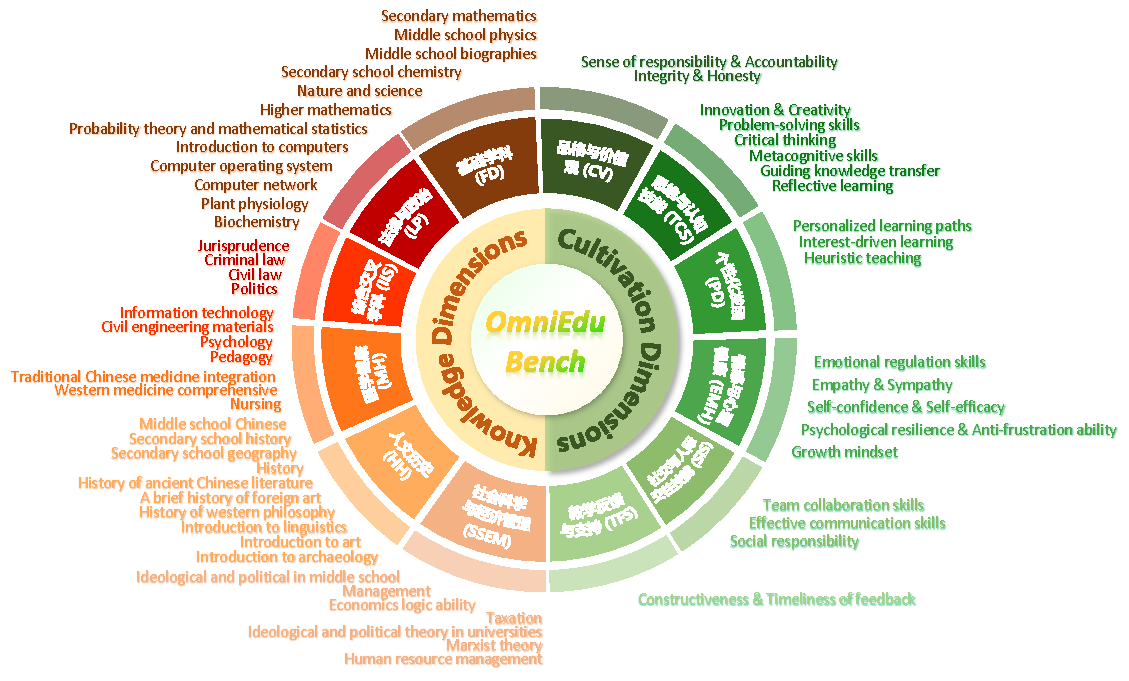
\includegraphics[height=0.6\textwidth]{figure/omniframe.pdf}
    \vspace{-8mm}
    \caption{Overview of OmniEduBench. The benchmark comprises two dimensions: 41 subjects across six categories in the knowledge, and 20 subjects across six categories in the cultivation.}
    \label{fig:omniframe}
    \vspace{-4mm}
\end{figure}